\section{Results}

We analyzed the short-term effects of \gls{RP} by examining accelerations and the position at the end of the 2.5-day arc. While the position is ultimately relevant for precise orbit determination, studying the accelerations in different scenarios and along the orbit can explain the cause of position changes. Additionally, the accelerations underscore differences between models of varying complexity.

To compare two accelerations over time, we used the \gls{RMSE}, which is defined as
\begin{align}
    \text{RMSE}(x, y) = \sqrt{\frac{1}{n}\sum_{i=1}^{n}\left(x_i - y_i\right)^2}.
\end{align}
The \gls{RMSE} describes the difference between two scalar time series $x_i, y_i$ and gives more weight to large deviations. These time series can be the magnitude of accelerations or individual components. The \gls{rRMSE} is defined as
\begin{align}
    \text{rRMSE}(x, y) = \sqrt{\frac{\sum_{i=1}^{n}\left(x_i - y_i\right)^2}{\sum_{i=1}^{n} y_i^2}}
\end{align}
and is useful to compare differences across orders of magnitude.

While the simulation evaluates accelerations in a global frame, the effect of accelerations on the orbit is best analyzed in a spacecraft-fixed coordinate system that is aligned with the orbital track. The RSW coordinate system is one such system, defined by the unit vectors~\cite{Vallado2013}
\begin{align}
    \vb R = \frac{\vb r}{\norm{\vb r}}, \quad
    \vb W = \frac{\vb r \times \vb v}{\norm{\vb r \times \vb v}},
    \quad \textrm{and} \quad \vb S = \vb W \times \vb R.
\end{align}
The radial component $\vb R$ is aligned with the planetocentric position vector $\vb r$. The cross-track component $\vb W$ is aligned with the angular momentum vector, or orbit plane normal, involving the linear velocity $\vb v$. The along-track component $\vb S$ completes the right-handed coordinate system. Note that $\vb S$ is generally not perfectly aligned with the velocity vector, only for circular orbits.





\subsection{Instantaneous reradiation}
\label{subsec:inst-rerad}

First, we investigated the effect of instantaneous reradiation for the paneled target model. This increases the acceleration proportional to each panel's $C_a$, normal to the panel (cf. \cref{eq:brdf-reaction-specular-diffuse-instrerad}).

\begin{figure}[t]
    \centering
    \begin{subfigure}[c]{\linewidth}
        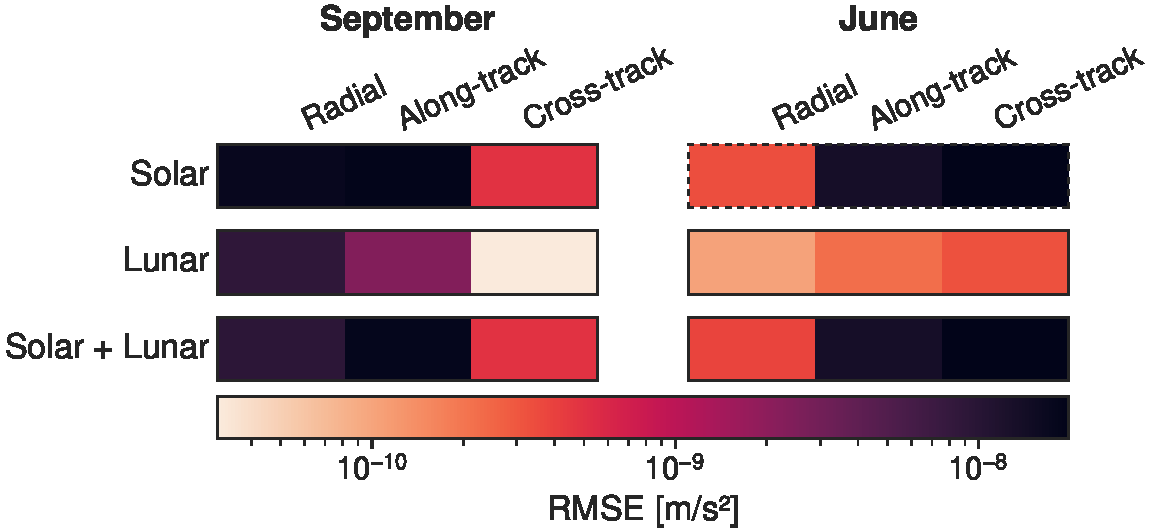
\includegraphics[width=\textwidth]{figures/plots/acc_reradiation_rms.pdf}
        \subcaption{Absolute}
     \end{subfigure}

     \bigskip

     \begin{subfigure}[c]{\linewidth}
        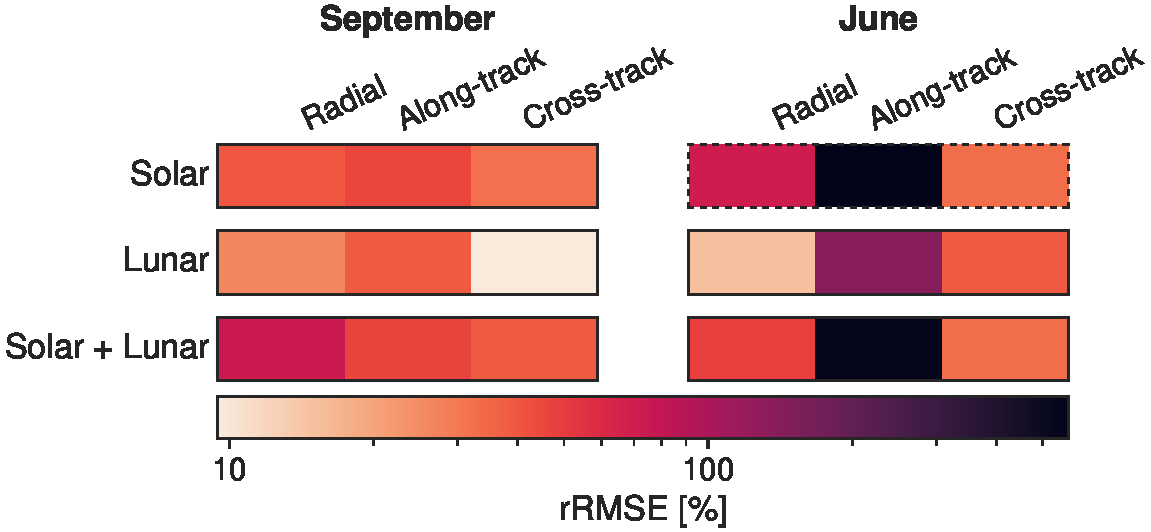
\includegraphics[width=\textwidth]{figures/plots/acc_reradiation_rrms.pdf}
        \subcaption{Relative}
     \end{subfigure}
    \caption{RMS differences of \gls{RP} accelerations over one orbit with and without instantaneous reradiation. The dashed boxes correspond to \cref{fig:acc-reradiation}.}
    \label{fig:acc-reradiation-rms}
\end{figure}

\begin{figure}[t]
    \centering
    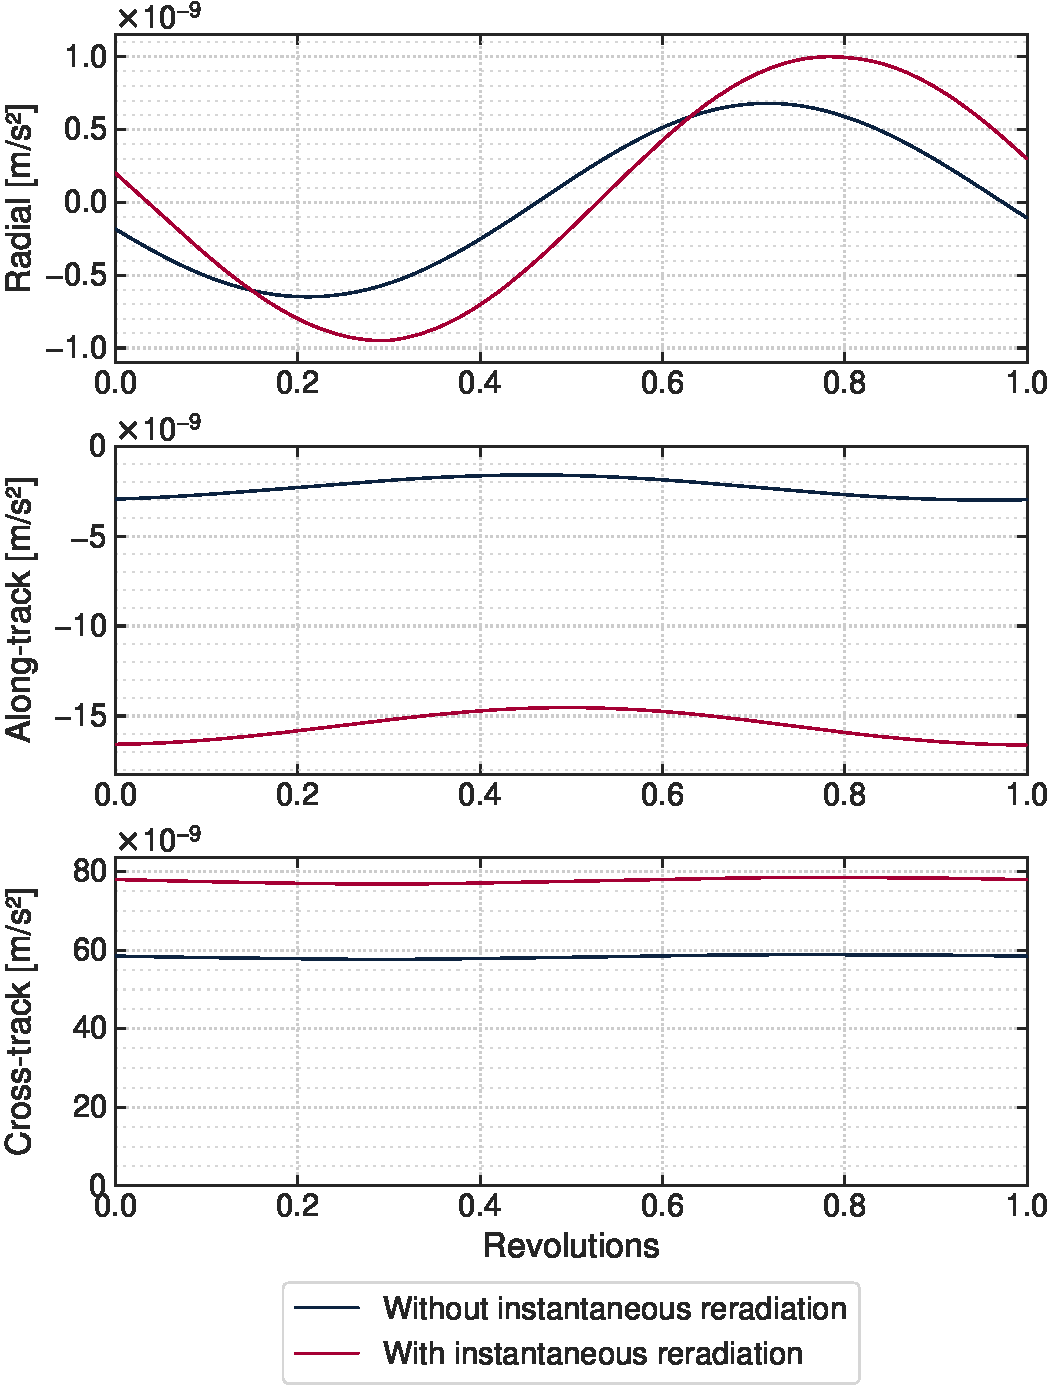
\includegraphics[width=\linewidth]{figures/plots/acc_reradiation_sun_jun.pdf}
    \caption{Accelerations due to solar radiation without and with instantaneous reradiation over one orbit for the June arc. There is a phase shift in the radial component and the along-track component increased by \qty{570}{\percent} \gls{RMSE}. Lunar contributions and the September arc are not significantly affected in shape.}
    \label{fig:acc-reradiation}
\end{figure}

\Cref{fig:acc-reradiation} shows the absolute and relative differences between accelerations without and with instantaneous reradiation. In absolute terms, the radial and along-track components are impacted most for the September arc, while the along-track and cross-track components experience the largest increase for the June arc (for both arcs, up to about \qty{1.9e-8}{\acc} \gls{RMSE}). The relative differences are more uniform (around \qty{40}{\percent} \gls{rRMSE}), but the along-track components of lunar and solar radiation in the June arc increase by \qty{140}{\percent} and \qty{570}{\percent} \gls{rRMSE}, respectively. In most cases, only the magnitude of accelerations changes but not the pattern.

\Cref{fig:acc-reradiation} shows the solar radiation of the June arc without and with instantaneous reradiation, the only of our simulations for which the pattern changed significantly. The phase of the radial acceleration is shifted by about \qty{10}{\percent} of the orbital period, which is not the case for the other two components or the acceleration due to lunar radiation. This arc also had the largest relative change in along-track acceleration as described above (highlighted in \cref{fig:acc-reradiation-rms}). This change manifests as a constant offset of about \qty{-13e-9}{\acc}. 

The large changes seen in some cases are mostly due to the +SA panel, which is highly absorptive ($C_a = 0.90$) and large ($A = \qty{11.00}{\m\squared}$). For the June arc, the solar array is angled at \qty{45}{\degree} with equal components in the cross-track and along-track directions The Sun is on the same side as the solar array in the cross-track direction. Without instantaneous reradiation, no panel has a significant contribution to the along-track acceleration, so it is quite small at around \qty{2e-9}{\acc}. With instantaneous reradiation, each panel, and especially the solar array, exerts an acceleration parallel to its normal, which leads to the along-track increase witnessed for the June arc.

We applied instantaneous reradiation for all of the following simulations since no reradiation due to spacecraft panels is physically unrealistic and the differences in magnitude are significant when instantaneous reradiation is added. More sophisticated thermal models involving conduction and internal heat generation would likely produce more accurate results.




% \subsection{Simulation setups}

% Solar with/without
% Lunar with/without
% Albedo none/constant/dlam
% Thermal none/angle-based
% LRO cannonball/paneled
% with/without isntantaneous reradiation
% Beta angle/arc

% 46 simulations





\subsection{Accelerations}
The most direct effect of \gls{RP} is visible in the accelerations. Therefore, we compare the \gls{RP} accelerations
\begin{itemize}
    \item for the September and June arcs,
    \item due to solar and lunar (albedo + thermal) radiation,
    \item for the constant and \gls{DLAM1} albedo distributions,
    \item for the cannonball and paneled targets.
\end{itemize}
In total, we ran 46 simulations. All accelerations are given in \qty{e-9}{\acc}. Regarding the cannonball and paneled target models, note that their comparative magnitudes are less important since the choice of cannonball parameters is somewhat arbitrary. Instead, we compared their behaviors and how they relate to model assumptions (e.g., symmetry for the cannonball, tracking for the paneled target).


\subsubsection{Solar and lunar radiation}
Both solar and lunar radiation are significant but their accelerations may amplify or cancel each other. To compare them, we used a constant albedo model in addition to the thermal model. The accelerations over one orbit are shown in \cref{fig:acc-solarvslunar}. Note that secular variations in orbit geometry can change the magnitude of acceleration components across orbits even within one 2.5-day arc but are not shown here.

\begin{figure*}[tb]
    \centering
    \begin{subfigure}[c]{\textwidth}
        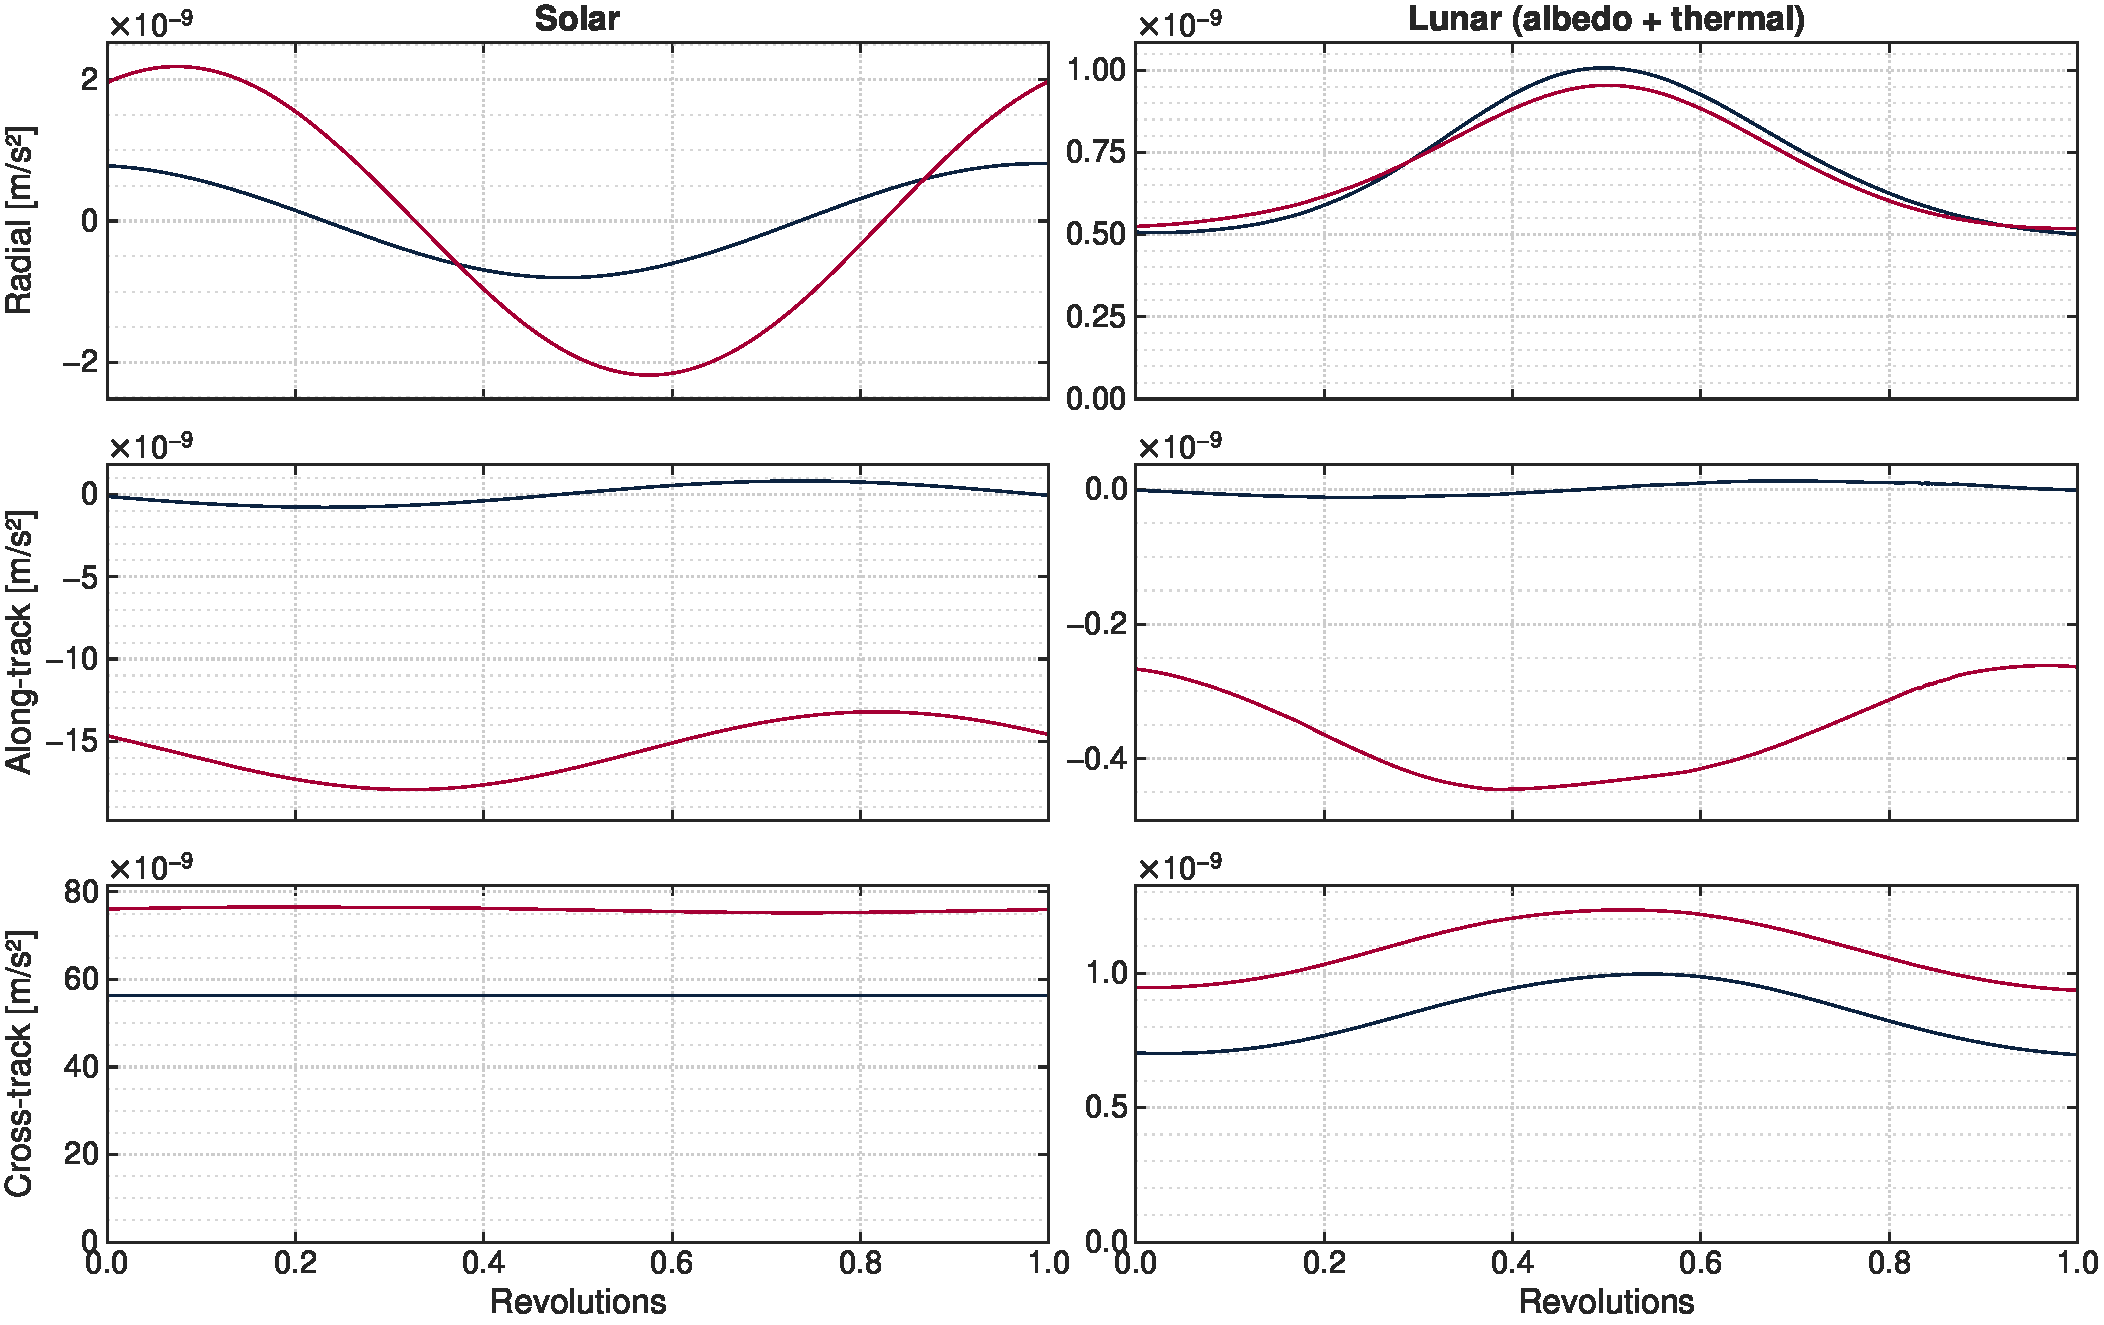
\includegraphics[width=\textwidth]{figures/plots/acc_solarvslunar_jun.pdf}
        \subcaption{June}
        \label{fig:acc-solarvslunar-jun}
     \end{subfigure}

     \bigskip

     \begin{subfigure}[c]{\textwidth}
        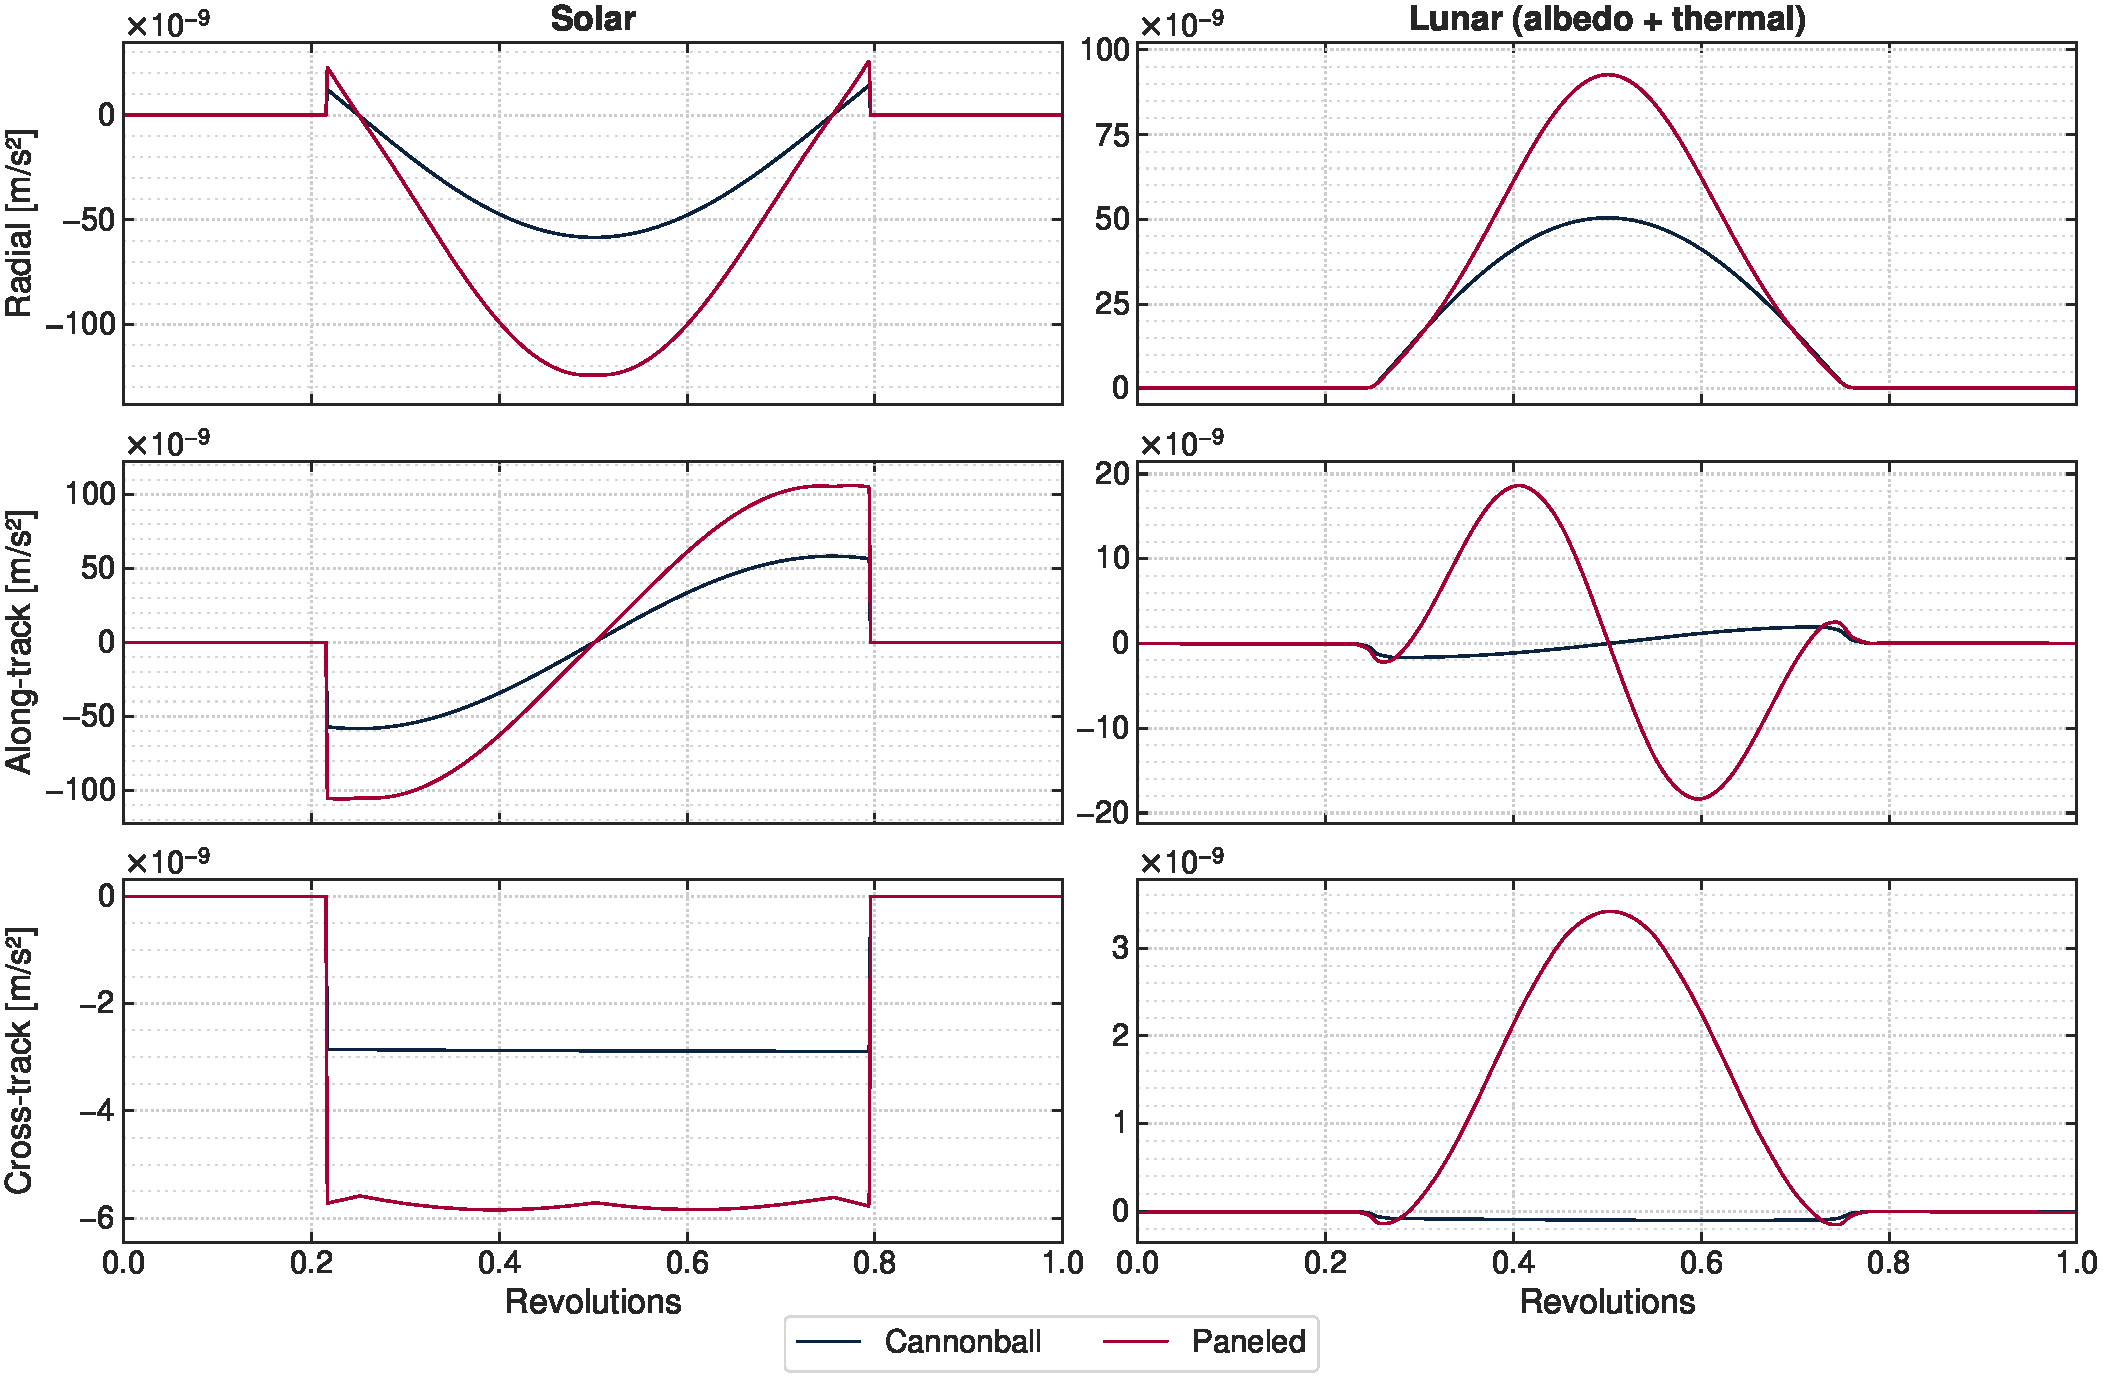
\includegraphics[width=\textwidth]{figures/plots/acc_solarvslunar_sep.pdf}
        \subcaption{September}
        \label{fig:acc-solarvslunar-sep}
     \end{subfigure}

    \caption{Accelerations due to solar and lunar radiation over one orbit. The cannonball and paneled targets differ both in magnitude and pattern of accelerations. Note the different scales of each subplot.}
    \label{fig:acc-solarvslunar}
\end{figure*}

For the June arc (\cref{fig:acc-solarvslunar-jun}), the spacecraft is in permanent sunlight and the orbit plane normal points toward the Sun because $\beta \approx \qty{90}{\degree}$. This leads to extremely large, constant cross-track solar accelerations. The paneled model also has along-track solar accelerations due to the solar array as explained in \cref{subsec:inst-rerad}. Interestingly, the radial solar accelerations show the same phase shift between the cannonball and paneled targets as observed without instantaneous reradiation (\cref{subsec:inst-rerad}). This suggests that symmetry, or the lack thereof, is the cause of the phase shift. The magnitude of the total solar acceleration does not change much throughout the year since it is only dependent on the Moon--Sun distance, which is relatively constant at \qty{1}{\astronomicalunit} (see \cref{tab:orbit-geometry}).

The lunar accelerations during the June arc are generally small (less than \qty{2}{\percent} of solar) because \gls{LRO} never passes over well-illuminated regions; half of the lunar source panels that are visible by \gls{LRO} are on the nightside and therefore rarely contribute. The sinusoidal variations in lunar radiation pressure are mainly caused by the fact that $\beta$ is not exactly \qty{90}{\degree} and \gls{LRO}'s angle to the subsolar point therefore varies by \qty{2}{\degree}. Periodic variations in altitude due to the eccentricity itself have a minimal effect since higher altitudes mean larger distances but also a larger visible area of the lunar surface, which roughly cancels. Secular variations in lunar accelerations (not shown) exist and are due to the evolution of eccentricity over the 2.5 days caused by the non-uniform lunar gravity field~\cite{Tooley2010}. The eccentricity ranges from 0.005 to 0.008, which leads to periselene altitudes between \qty{37}{\km} and \qty{41}{\km}. Such changes in eccentricity lead to larger amplitudes but no mean shift.

For the September arc (\cref{fig:acc-solarvslunar-sep}), the Sun is occulted for \qty{42}{\percent} of the orbit since $\beta \approx \qty{0}{\degree}$. The effect of these occultations is evident in solar and lunar radiation, both of which vanish on the nightside. The accelerations are mostly in the radial and along-track directions. This is most clearly explained by the solar accelerations: At 0.2, \gls{LRO} crosses the terminator above the pole and is moving straight toward the Sun; the along-track component is then maximal and negative since the Sun opposes the spacecraft's motion. Continuing the orbit, \gls{LRO} passes above the subsolar point at 0.5, leading to a maximal and negative radial component while the along-track component has vanished. Further toward the other pole, \gls{LRO} passes into the night at 0.8, where the along-track component accelerates the spacecraft into the direction of motion. During this whole time, the cross-track component is slightly negative because $\beta$ is slightly negative but not zero. If $\beta$ were slightly positive, the cross-track component would be similar but with the sign flipped. In addition to periodic changes, there is a secular change in solar accelerations (not shown) since the already slightly negative $\beta$ continues to decrease: over the 2.5-day arc, the mean of the along-track and cross-track components increase twofold and threefold, respectively. This trend continues until the cross-track component dominates for high $\beta$, as seen for the June arc.

The lunar accelerations during the September arc are much larger than during the June arc because \gls{LRO} passes right over the subsolar point, which reflects much sunlight and has high thermal emissions. Indeed, the lunar irradiance (up to \qty{1831}{\irr}) is larger than the solar irradiance (up to \qty{1362}{\irr}) above the subsolar point. Still, the lunar acceleration magnitude is \qty{14}{\percent} smaller than the solar acceleration magnitude since lunar panels are distributed azimuthally around the nadir and thus partially cancel while all solar rays are parallel. Another feature of lunar accelerations is the sign opposite to solar accelerations: when passing over the subsolar point, the radial components of solar and lunar accelerations roughly cancel. A similar effect can be seen in the along-track and cross-track components for a paneled target, although the lunar radiation needs some time to build up: The along-track component peaks at a subsolar angle of \qty{33}{\degree}, the cross-track component above the subsolar point. The cross-track component increases secularly over the 2.5-day arc, similarly to solar radiation.

Comparing the accelerations of cannonball and paneled targets for both arcs, it is clear that a single $C_r$ cannot capture the complex and changing spacecraft geometry. While the solar accelerations for the September arc are just off by about a constant factor, this is not the case for the June arc or any of the lunar accelerations. In fact, the sign may even be different, particularly for lunar along-track and cross-track accelerations in September. This is likely caused by the solar array tracking the Sun. On smaller scales, the effect of target panels of different sizes and reflective properties becoming illuminated as \gls{LRO} revolves around the Moon can be seen in the kinks of the solar cross-track accelerations of the September arc.

All accelerations are inversely proportional to the spacecraft's mass. While we chose the end-of-mission mass for all simulations, the begin-of-mission mass is \qty{17}{\percent} higher and all accelerations are thus \qty{17}{\percent} lower (see \cref{subsec:lro-target}). This only changes magnitudes, not patterns.





\subsubsection{Lunar albedo and thermal radiation}
In the previous subsection, lunar radiation was considered as the sum of albedo and thermal radiation. In this subsection, we look at the separate contributions and the differences between albedo distributions. The accelerations on a paneled target are shown in \cref{fig:acc-albedovsthermal}.

\begin{figure*}[tb]
    \centering
    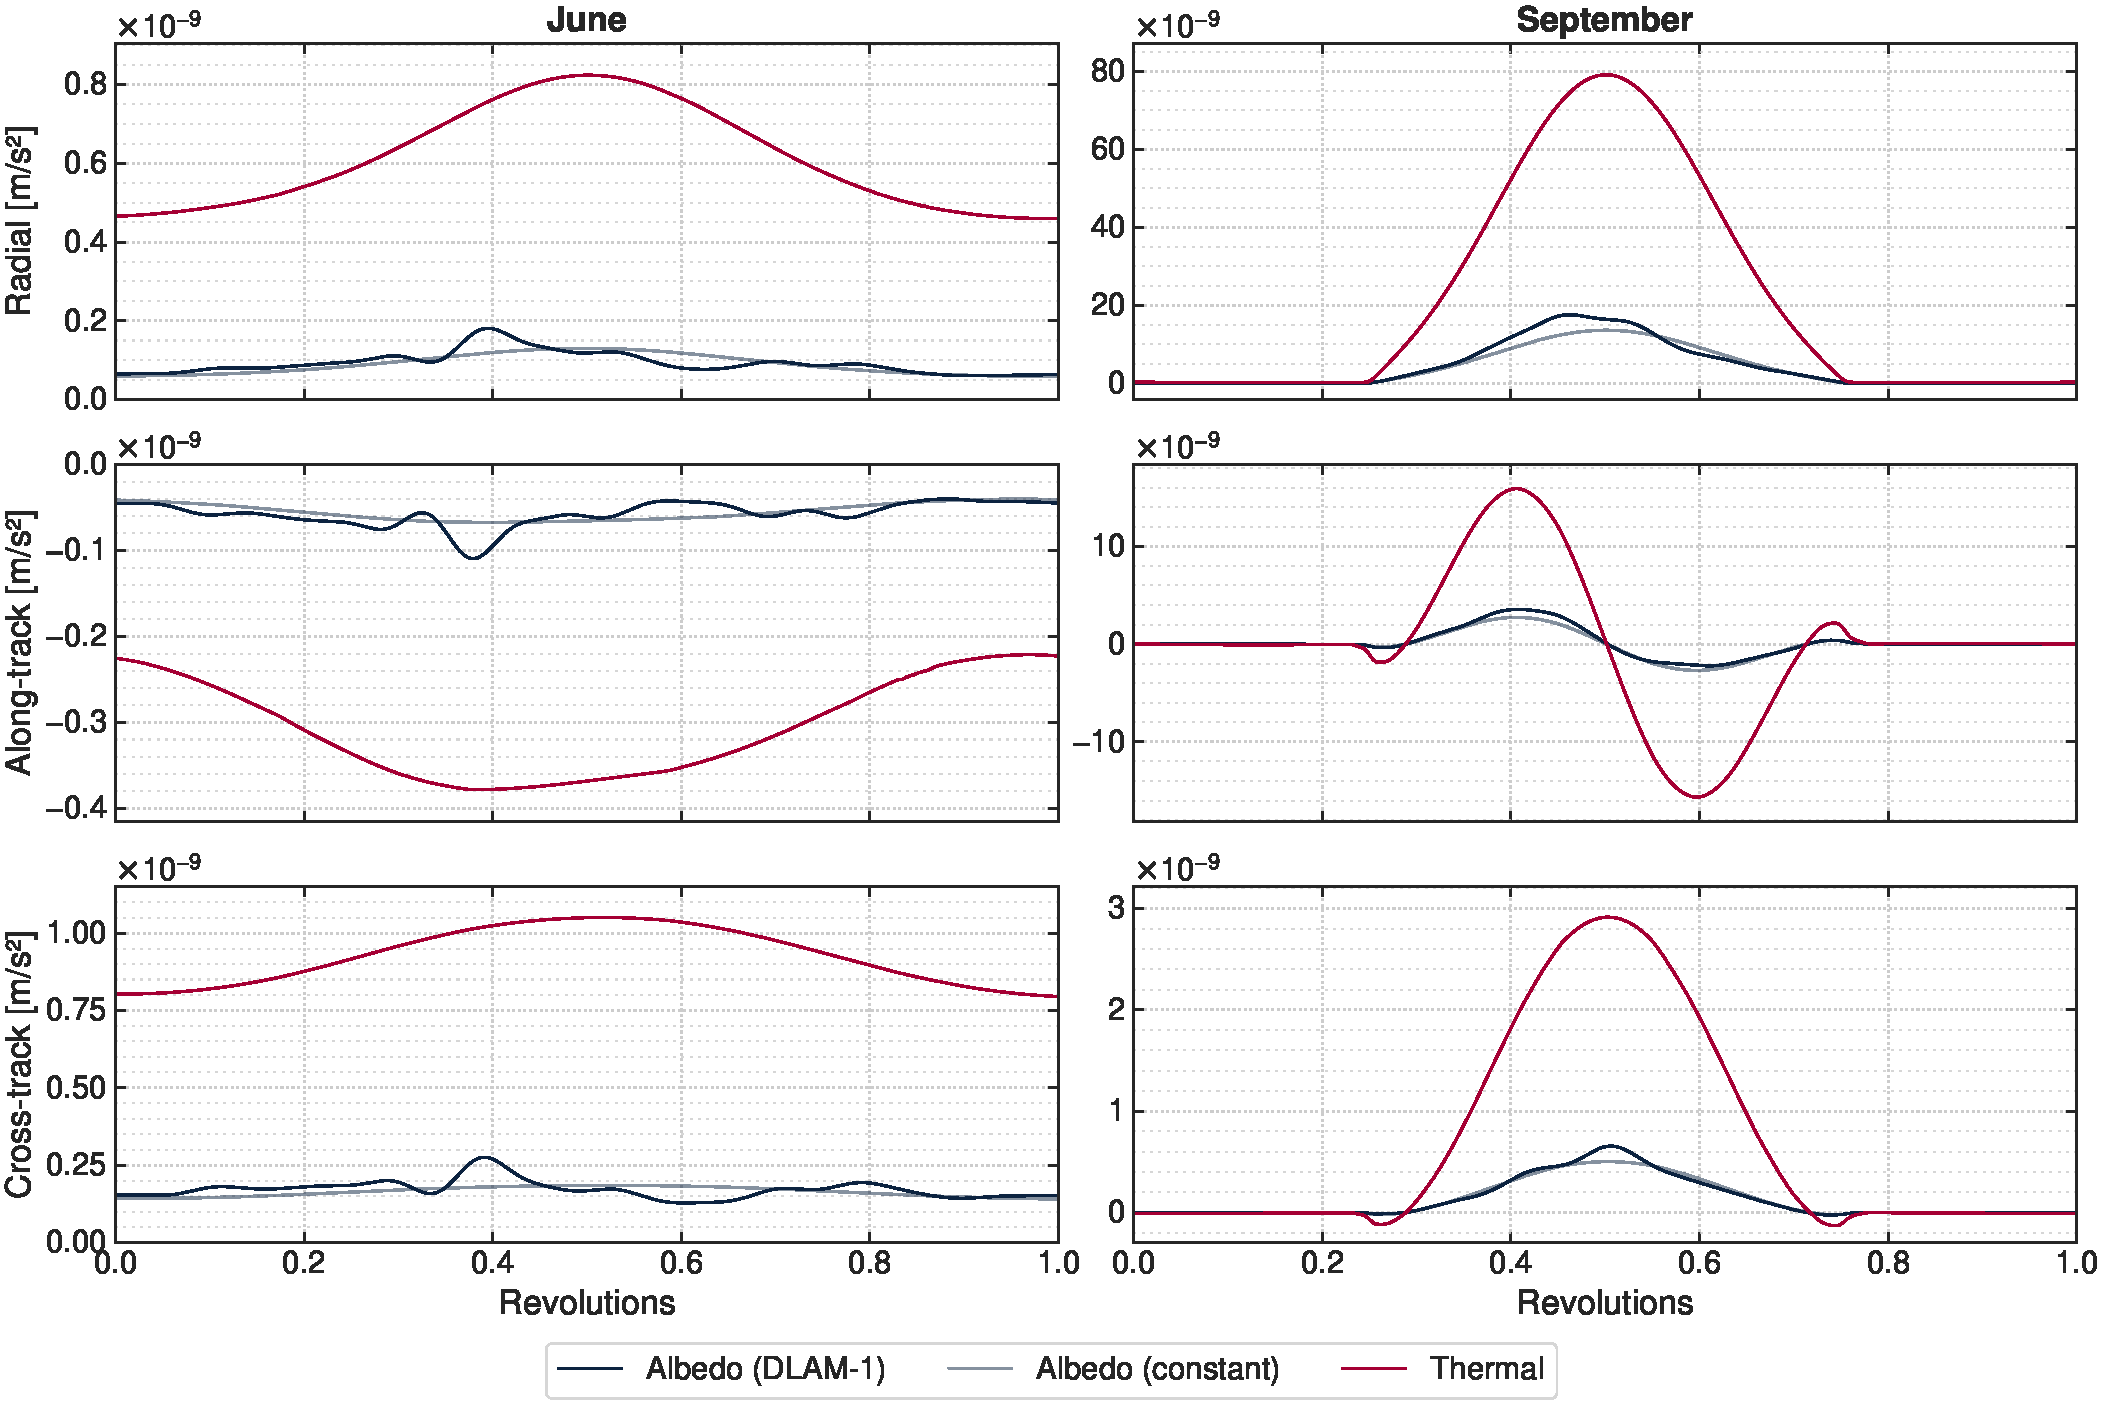
\includegraphics[width=\textwidth]{figures/plots/acc_albedovsthermal.pdf}

    \caption{Accelerations due to lunar thermal and albedo radiation on a paneled target. Thermal radiation dominates at all times and the difference between constant and \gls{DLAM1} albedo is small. Note the different scales of each subplot.}
    \label{fig:acc-albedovsthermal}
\end{figure*}

For both arcs and all components, thermal radiation is far larger than albedo radiation (up to sixfold). This is even though the albedo is likely overestimated by \qty{25}{\percent} as described in \cref{subsec:lunar-albedo}. In terms of behavior, the thermal radiation and constant albedo radiation are very similar: smooth and dependent on the subsolar angle. However, albedo radiation vanishes in the eclipse region of the September arc. The thermal irradiance at \gls{LRO} on the nightside is \qty{6}{\irr}, which leads to a small total acceleration of \qty{1e-9}{\acc}.


\begin{figure}[htb]
    \centering
    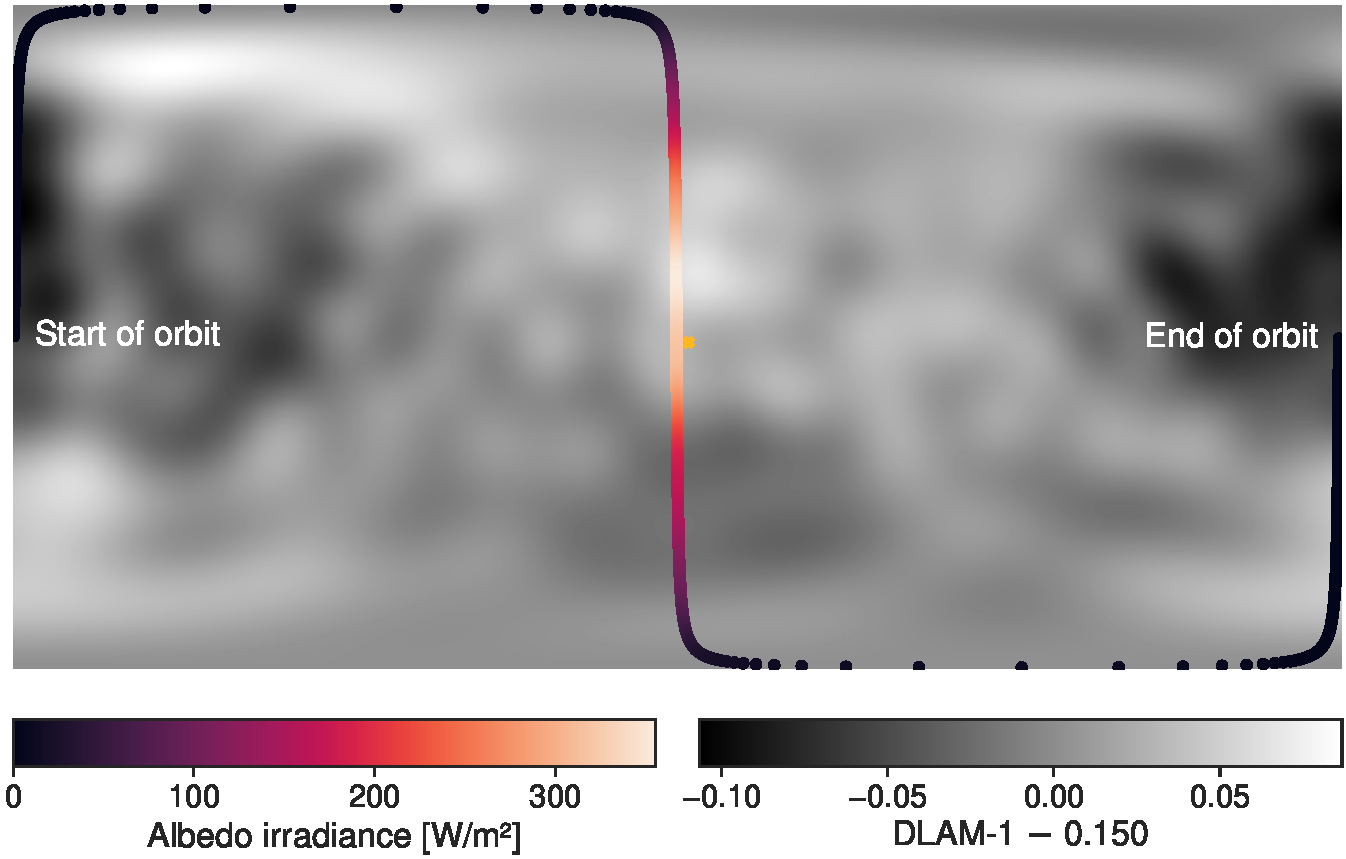
\includegraphics[width=\linewidth]{figures/plots/groundtrack.pdf}
    \caption{Ground track for September arc, colored by the irradiance due to \gls{DLAM1} albedo. The map shows the difference between \gls{DLAM1} and the constant albedo ($a=0.150$). The maximum irradiance does not occur above the subsolar point (\textcolor{mpl-yellow}{\ding{54}}) but above the local albedo maximum \qty{18}{\degree} north of it.}
    \label{fig:groundtrack}
\end{figure}

The accelerations of the constant and \gls{DLAM1} albedo distributions are of very similar magnitude (in non-zero regions, rRMSE of \qty{19}{\percent} for June and \qty{24}{\percent} for September), although \gls{DLAM1} exihibits irregular variations. The largest difference of \qty{5e-9}{\acc} occurs in the radial component for the September arc at about 0.55. Interestingly, \gls{DLAM1} albedo radiation peaks \emph{before} the subsolar point, where the thermal and constant albedo radiation peak. This behavior can be explained by the ground track of this orbit. \Cref{fig:groundtrack} shows the \gls{DLAM1} albedo irradiance along the ground track over a map of the difference between \gls{DLAM1} and the constant albedo. In this figure, the maximum albedo difference also appears before the subsolar point and coincides with a region where \gls{DLAM1} has an albedo that is \num{0.067} higher or \qty{55}{\percent} more reflective than the constant albedo of $a=0.150$. All irregular differences between the albedo distributions seen in \cref{fig:acc-albedovsthermal} are explained by this map. However, because the thermal radiation is so much larger, the effect of these differences remains overall limited.








\subsection{Change in final position}
The goal of orbit determination is to estimate the state, and particularly the position, of a spacecraft over time. Therefore, the difference in position at the end of the arc between models is highly relevant. As mentioned in \cref{sec:introduction}, the maximum allowable error is \qtyrange{50}{100}{\m} in total position and below \qty{1}{\m} radially. Since the true position is not known and this paper is rather concerned with relative differences, we use a simulation without solar and lunar radiation as a baseline reference.

\begin{table*}[tb]
    \caption{Difference of final position in \unit{\m} with respect to the no-\gls{RP} baseline, given as mean over the final orbit plus/minus periodic variations around that mean. The largest changes are in the along-track position. $\mathbf{A}$: solar only; $\mathbf{B}$: lunar only (thermal + constant albedo); $\mathbf{C}$: lunar only (thermal + \gls{DLAM1} albedo); $\mathbf{D}$: solar + lunar (thermal + \gls{DLAM1} albedo).}
    \label{tab:final-position}
    \begin{subtable}[c]{\textwidth}
        \begin{tabular}{llllllllll}
\toprule
 & \multicolumn{4}{c}{\bfseries Cannonball} & \bfseries  & \multicolumn{4}{c}{\bfseries Paneled} \\
 & Radial & Along-track & Cross-track & RMSE &  & Radial & Along-track & Cross-track & RMSE \\
\cmidrule{2-5}\cmidrule{7-10}
\bfseries A & $\num{+0.0 \pm 0.2}$ & $\num{-0.5 \pm 0.5}$ & $\num{+0.1 \pm 0.1}$ & $\num{0.6}$ & ~ & $\num{-7.5 \pm 6.7}$ & $\num{+1066.1 \pm 39.3}$ & $\num{+0.1 \pm 0.2}$ & $\num{1033.5}$ \\
\bfseries B & $\num{+0.0 \pm 0.0}$ & $\num{-0.3 \pm 0.0}$ & $\num{+0.0 \pm 0.0}$ & $\num{0.3}$ & ~ & $\num{-0.2 \pm 0.2}$ & $\num{+24.4 \pm 0.9}$ & $\num{+0.0 \pm 0.0}$ & $\num{23.6}$ \\
\bfseries C & $\num{+0.0 \pm 0.0}$ & $\num{-0.3 \pm 0.0}$ & $\num{+0.0 \pm 0.0}$ & $\num{0.3}$ & ~ & $\num{-0.2 \pm 0.2}$ & $\num{+24.6 \pm 0.9}$ & $\num{+0.0 \pm 0.0}$ & $\num{23.9}$ \\
\bfseries D & $\num{+0.0 \pm 0.2}$ & $\num{-0.8 \pm 0.4}$ & $\num{+0.1 \pm 0.1}$ & $\num{0.8}$ & ~ & $\num{-7.7 \pm 6.9}$ & $\num{+1090.7 \pm 40.2}$ & $\num{+0.1 \pm 0.2}$ & $\num{1057.4}$ \\
\bottomrule
\end{tabular}

        \subcaption{June}
     \end{subtable}

     \medskip

     \begin{subtable}[c]{\textwidth}
        \begin{tabular}{llllllllll}
\toprule
 & \multicolumn{4}{c}{\bfseries Cannonball} & \bfseries  & \multicolumn{4}{c}{\bfseries Paneled} \\
 & Total & Radial & Along & Cross &  & Total & Radial & Along & Cross \\
\cmidrule{2-5}\cmidrule{7-10}
\bfseries Solar only & $60.9_{-24.9}^{+23.9}$ & $0.2_{-12.1}^{+12.4}$ & $-36.4_{-25.1}^{+23.8}$ & $0.0_{-0.4}^{+0.5}$ & ~ & $108.3_{-48.1}^{+45.1}$ & $0.3_{-23.0}^{+23.7}$ & $-61.8_{-47.7}^{+45.6}$ & $0.0_{-0.9}^{+0.9}$ \\
\bfseries Lunar only (constant) & $7.4_{-5.4}^{+5.8}$ & $0.1_{-2.9}^{+2.8}$ & $-12.2_{-5.9}^{+5.2}$ & $0.0_{-0.1}^{+0.1}$ & ~ & $2.4_{-11.6}^{+11.2}$ & $0.1_{-6.1}^{+5.9}$ & $-11.6_{-12.4}^{+11.4}$ & $0.0_{-0.2}^{+0.2}$ \\
\bfseries Lunar only (DLAM-1) & $7.7_{-5.5}^{+5.9}$ & $0.1_{-2.9}^{+2.8}$ & $-12.6_{-6.0}^{+5.3}$ & $0.0_{-0.1}^{+0.1}$ & ~ & $10.8_{-11.8}^{+12.5}$ & $0.1_{-6.2}^{+6.1}$ & $-21.4_{-12.9}^{+11.3}$ & $0.0_{-0.2}^{+0.2}$ \\
\bfseries Solar + lunar (DLAM-1) & $68.4_{-18.2}^{+19.3}$ & $0.2_{-9.2}^{+9.5}$ & $-49.1_{-19.8}^{+17.8}$ & $0.0_{-0.4}^{+0.4}$ & ~ & $118.7_{-33.6}^{+35.4}$ & $0.4_{-17.0}^{+17.5}$ & $-83.2_{-36.3}^{+32.7}$ & $0.0_{-0.6}^{+0.6}$ \\
\bottomrule
\end{tabular}

        \subcaption{September}
     \end{subtable}
\end{table*}

The differences in final positions with respect to the baseline simulation are shown in \cref{tab:final-position}. The first number is the mean, secular difference over the final orbit (32nd revolution), and the second number gives the amplitude of periodic variations around that mean over the final orbit. Note that the periodic variation is quite large in some cases despite zero secular change.

The June arc shows a large along-track difference (more than \qty{1}{\km}) for the paneled target with solar radiation ($\mathbf{A}$). This is likely due to accumulation of the consistently large along-track acceleration of about \qty{-15e-9}{\acc}. However, this acceleration is of lower magnitude than the constant acceleration of \qty{+47e-9}{\acc} expected to result in this position difference, and of the opposite sign. For the cannonball, the along-track accelerations have a zero mean and thus the position difference is also zero. This, again, reveals how the cannonball cannot account for asymmetry; with symmetric accelerations, no secular changes occur. Interestingly, the large cross-track acceleration does not lead to a large cross-track difference in the final position. Possibly, along-track accelerations have the greatest effect since they are almost aligned with the large orbital velocity (\qty{1.7}{\km\per\s}). Constant and \gls{DLAM1} albedo ($\mathbf{B}$ and $\mathbf{C}$) do not differ significantly.

For the September arc, the cannonball and paneled targets give more similar results. Again, the largest secular difference is in the along-track position. However, in contrast to the June arc, \gls{LRO} is shifted back in the track this time. Due to the large variations in radial and along-track accelerations over each orbit, there are large periodic variations in the radial and along-track positions too. For the paneled target with solar and lunar radiation ($\mathbf{D}$), these have amplitudes of \qty{18}{\m} and \qty{36}{\m} for the radial and along-track differences, respectively. The periodic variations have higher amplitudes when not including lunar radiation ($\mathbf{A}$), which would otherwise cancel solar accelerations partially. There also is an \qty{8}{m} RMSE difference for the paneled model between constant and \gls{DLAM1} albedo, the only case where the choice of albedo model influences the final position.


These differences in position emphasize the importance of \gls{RP} models for precise orbit determination. The best estimate of the true effect of \gls{RP} is given by setup $\mathbf{D}$ (solar + lunar radiation) for the paneled target. For both arcs, the maximum allowable total error would be exceeded by the sum of secular and periodic variations if \gls{RP} were neglected. The radial requirement of sub-meter accuracy would be violated by periodic variations alone.




% \subsection{Change in orbital element}

% No good results since Tudat calculates elements from propagation frame, not Moon frame

% \begin{landscape}
    
%     \begin{table}
%         \small
%         \caption{Difference of Kepler elements with respect to no-\gls{RP} baseline, given as mean over the final orbit. The elements are the semi-major axis ($a$ in \unit{m}), eccentricity ($e$, unitless), inclination ($i$ in \unit{\degree}), longitude of the ascending node ($\Omega$ in \unit{\degree}), and argument of periapsis ($\omega$ in \unit{\degree}).}
%         \label{tab:final-elements}
%         \begin{subtable}[c]{\textwidth}
%             \begin{tabular}{llllllllllll}
\toprule
 & \multicolumn{5}{c}{\bfseries Cannonball} & \bfseries  & \multicolumn{5}{c}{\bfseries Paneled} \\
 & $a$ & $e$ & $i$ & $\Omega$ & $\omega$ &  & $a$ & $e$ & $i$ & $\Omega$ & $\omega$ \\
\cmidrule{2-6}\cmidrule{8-12}
\bfseries Solar only & \num{+0.0015} & \num{+8.3e-10} & \num{+1.2e-06} & \num{-1.8e-06} & \num{+0.001} & ~ & \num{-7.2} & \num{-2.6e-07} & \num{+7.1e-06} & \num{+5.3e-06} & \num{+0.0022} \\
\bfseries Lunar only (constant) & \num{+7.4e-05} & \num{+5.7e-10} & \num{-1.2e-07} & \num{+1.8e-07} & \num{-7.2e-05} & ~ & \num{-0.17} & \num{-8.6e-09} & \num{+8.8e-08} & \num{+3.9e-07} & \num{-4.8e-05} \\
\bfseries Lunar only (DLAM-1) & \num{+7.6e-06} & \num{-1.9e-10} & \num{-6.4e-08} & \num{+2.1e-07} & \num{-7.3e-05} & ~ & \num{-0.17} & \num{-9.4e-09} & \num{+1.6e-07} & \num{+4.2e-07} & \num{-4.1e-05} \\
\bfseries Solar + lunar (DLAM-1) & \num{+0.0015} & \num{+6.4e-10} & \num{+1.2e-06} & \num{-1.6e-06} & \num{+0.00097} & ~ & \num{-7.4} & \num{-2.7e-07} & \num{+7.2e-06} & \num{+5.7e-06} & \num{+0.0021} \\
\bottomrule
\end{tabular}

%             \subcaption{June}
%          \end{subtable}
    
%          \medskip
    
%          \begin{subtable}[c]{\textwidth}
%             \begin{tabular}{llllllllllll}
\toprule
 & \multicolumn{5}{c}{\bfseries Cannonball} & \bfseries  & \multicolumn{5}{c}{\bfseries Paneled} \\
 & $a$ & $e$ & $i$ & $\Omega$ & $\omega$ &  & $a$ & $e$ & $i$ & $\Omega$ & $\omega$ \\
\cmidrule{2-6}\cmidrule{8-12}
\bfseries Solar only & \num{+0.23} & \num{-5.8e-06} & \num{+5.7e-06} & \num{+1.3e-05} & \num{-0.027} & ~ & \num{+0.4} & \num{-1.1e-05} & \num{+1.1e-05} & \num{+2.6e-05} & \num{-0.052} \\
\bfseries Lunar only (constant) & \num{+0.039} & \num{+1.3e-06} & \num{+1.4e-07} & \num{-3.1e-06} & \num{+0.0062} & ~ & \num{+0.039} & \num{+2.8e-06} & \num{-4.1e-06} & \num{-6.5e-06} & \num{+0.013} \\
\bfseries Lunar only (DLAM-1) & \num{+0.041} & \num{+1.3e-06} & \num{+1.6e-07} & \num{-3.1e-06} & \num{+0.0061} & ~ & \num{+0.1} & \num{+2.8e-06} & \num{-4.3e-06} & \num{-6.6e-06} & \num{+0.013} \\
\bfseries Solar + lunar (DLAM-1) & \num{+0.27} & \num{-4.4e-06} & \num{+5.8e-06} & \num{+1e-05} & \num{-0.021} & ~ & \num{+0.5} & \num{-8.2e-06} & \num{+6.6e-06} & \num{+1.9e-05} & \num{-0.038} \\
\bottomrule
\end{tabular}

%             \subcaption{September}
%          \end{subtable}
%     \end{table}

% \end{landscape}

% compare wih Gauss perturbing equations (analytical solution to change of osculating elements based on accelerations), e.g. ~\cite[Sec.~3.2]{Lucchesi2006}

% Keplerian state wrt ECLIPJ2000, not Moon frame!!

% prediction september: change in arg peri because solar along-track acts fully above poles without being cancelled by lunar rad

% for september: sign of change of inclination and lon asc node depends on sign of beta




\subsection{Performance}
Choosing the appropriate model is not only a consideration of accuracy but also one of computational effort. The aim is to find the most efficient model that is sufficiently accurate. To determine how much less efficient complex models like paneled targets or \gls{DLAM1} are, we measured wall time durations for different model combinations. We ran each simulation 100 times in random order on a server with 2 Intel Xeon E5-2683 v3 CPUs (14 cores, two threads per core with hyperthreading) while no other loads were present. 27 simulations ran in parallel such that all but one core were used by. More parallelism would have triggered hyperthreading, which could have skewed measurements. \gls{Tudat} was compiled in release configuration with GCC 11.4.0 at optimization level \texttt{-O2}. No other steps such as CPU pinning were taken. Note that software performance can be influenced by many, seemingly innocuous aspects~\cite{Mytkowicz2009}. Still, the results show the general tendency.

\begin{figure}[b]
    \centering
    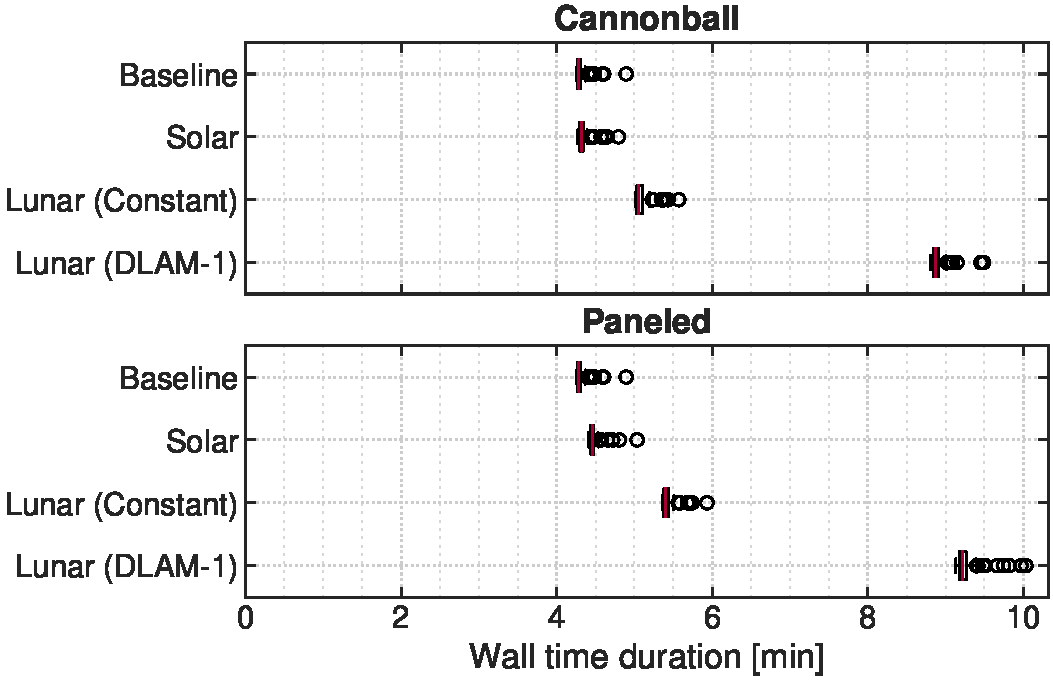
\includegraphics[width=\linewidth]{figures/plots/performance.pdf}
    \caption{Wall time duration of simulations with different \gls{RP} models. The statistics come from 100 runs for each model. Evaluation of \gls{DLAM1}'s spherical harmonics expansion increases the duration by up to \qty{80}{\percent}.}
    \label{fig:performance}
\end{figure}

The wall time durations when including solar or lunar radiation are shown in \cref{fig:performance}. Again, the baseline simulation without radiation serves as a reference. The median baseline time of \qty{4.3}{\min} includes computations of the lunar spherical harmonics gravity model, point gravities from Sun and Earth, and general integration and propagation. Solar radiation has a negligible complexity, even for a paneled target. Lunar radiation with constant albedo increases the duration by about \qty{20}{\percent}, but slightly more for the paneled than the cannonball target. Taking the albedo from the spherical harmonics expansion of \gls{DLAM1} increases the duration by up to \qty{80}{\percent} compared to the baseline. This is a significant performance penalty, which may not always be tolerable. Other authors even report increases of several hundred percent for \gls{DLAM1} albedo~\cite{Nicholson2010}.

The durations are relatively consistent as indicated by the inter-quartile range of at most \qty{5}{\s}. Still, all distributions have a long tail toward longer durations: the difference between maximum and median is between 9 and 21 times higher than the difference between minimum and median. This skewness is typical for software performance.
